\chapter{Zielsetzung}

Bei dem Projekt "`Sportangebot der HTW"' ging es darum, einen Beratungsassistenten zu erstellen. Hierbei handelt es sich um ein Softwareprodukt, das auf Fragestellungen Sportinteressierten nach Beantwortung eine geeignete Sportart vorschlägt.

\section{Szenarien}

Als Testfall wurden zwei Szenarien aufgestellt. Bei den Szenarien wurden bereits Überlegungen getroffen, ob die Fragen durch die Ontologie oder durch die Datenbank gefiltert werden nach der Natur der Sache. Bei der Umsetzung wurden allerdings teilweise veränderungen vorgenommen. Dazu später mehr.

Die folgenden Abbildungen (\ref{fig:Szenario 1} und \ref{fig:Szenario 2}) stellen die Szenarien dar, wie sie das Team zum Zeitpunkt des ersten Meilensteins ausgearbeitet hat.

\begin{capfigure}[Szenario 1]
	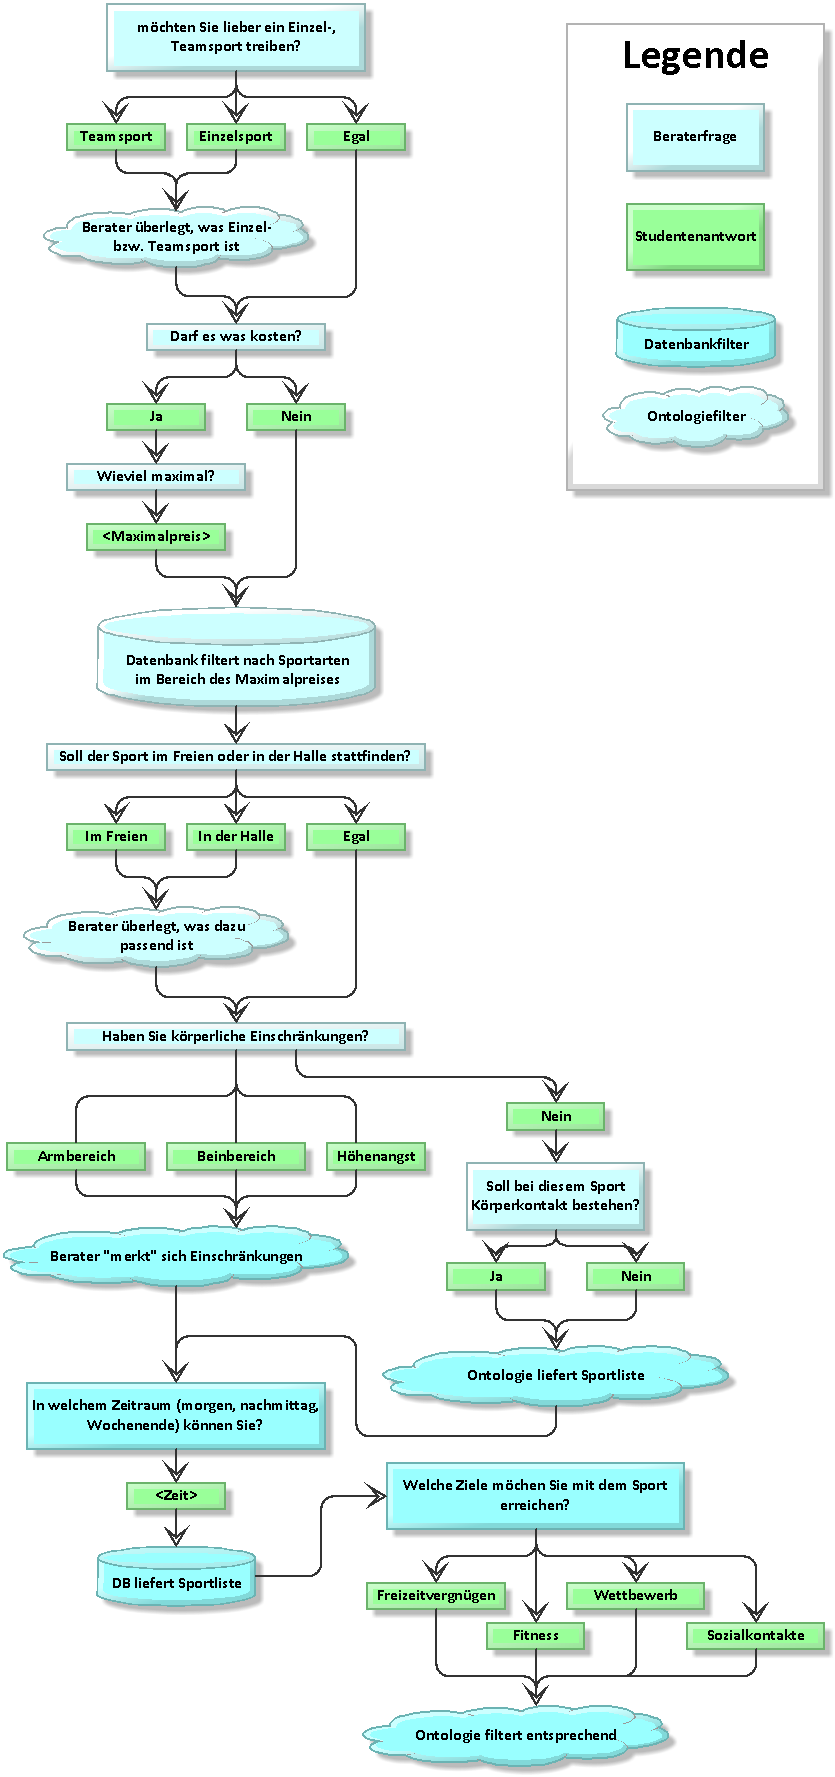
\includegraphics[width=100mm]{images/szenario1.png}
\end{capfigure}

\begin{capfigure}[Szenario 2]
	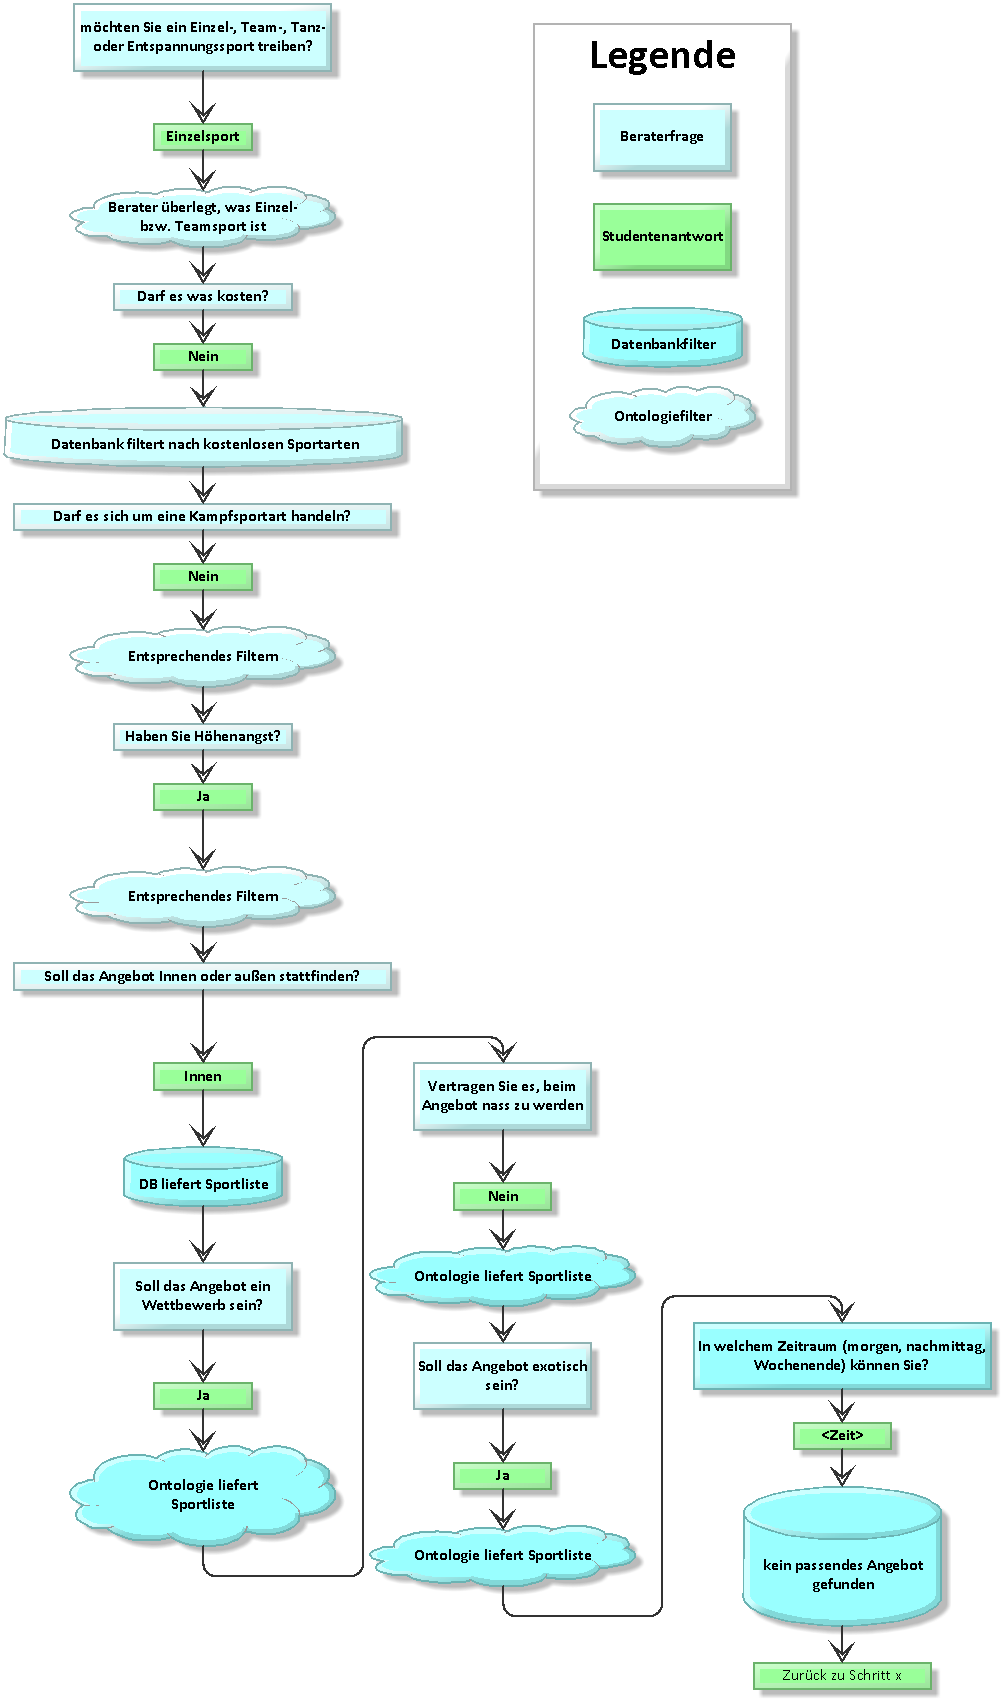
\includegraphics[width=100mm]{images/szenario2.png}
\end{capfigure}






% DONE \TODO{[PRIO:NORMAL]Tabellen sind so nicht sonderlich intuitiv und definitiv nicht schön. Hier wäre eine andere Variante der Darstellung besser. Idealerweise eine, die die Wege anzeigt.}
